% =====================================================================
%  LaTeX preamble for the Farsi MRI book (PDF output via XeLaTeX)
%  Injected by Quarto as `include-in-header` for the PDF format.
%
%  Bidi strategy: babel + bidi=basic
%  ---------------------------------
%  We make the document right-to-left with `babel`'s built-in bidi engine
%  (`bidi=basic`), which uses the LaTeX kernel's bidi support. This is more
%  robust with modern `array`/`longtable`/`booktabs` than the older `bidi`
%  package (used by polyglossia/xepersian), which patches tabular internals
%  and breaks on current `array` (missing \UseMathForPositioningText).
%
%  * Persian is the main language (RTL); `english` is available for LTR runs.
%  * \babelsublr{...} forces a left-to-right "island" — see theme/ltr.lua.
%  * Math ($...$) and verbatim/code stay LTR automatically.
%  * The body font is set here via \babelfont (loaded by file from fonts/),
%    so DO NOT also set `mainfont` in _quarto.yml for PDF.
%
%  NOTE: anything that loads packages (tikz, pgfplots, …) is fine before or
%  after babel here; bidi=basic does not impose a "load last" rule.
% =====================================================================

% --- TikZ / PGF for inline vector diagrams (also used by diagrams/). --------
\usepackage{tikz}
\usepackage{pgfplots}
\pgfplotsset{compat=1.18}
\usetikzlibrary{arrows.meta}

% --- Math packages the chapters rely on. -----------------------------------
% mathtools pulls in amsmath and adds \xleftrightarrow, \coloneqq, \xmapsto, …
% (amsmath/amssymb are already loaded by Quarto; \boldsymbol comes from there.)
% NOTE: do NOT add siunitx/bm here — they remap \mu and break \boldsymbol\mu.
\usepackage{mathtools}

% --- RTL / Persian via babel (bidi=basic) -----------------------------------
\usepackage[bidi=basic]{babel}
\babelprovide[import]{english}
\babelprovide[main, import]{persian}
% Body font (Vazirmatn) loaded by file — no system font install needed.
% Set BOTH roman and sans to Vazirmatn: KOMA renders the title and headings
% in the sans family, so the sans face must also cover Persian glyphs
% (otherwise the title/headings show as empty boxes / tofu).
% Renderer=Node forces luaotfload's stable node shaper instead of HarfBuzz.
% (LuaHBTeX defaults to HarfBuzz, which has an assertion bug on some Persian
% glyph sequences in the content; the node renderer shapes Persian correctly.)
\babelfont{rm}[Renderer=Node, Path=fonts/, Extension=.ttf, UprightFont=*-Regular, BoldFont=*-Bold]{Vazirmatn}
\babelfont{sf}[Renderer=Node, Path=fonts/, Extension=.ttf, UprightFont=*-Regular, BoldFont=*-Bold]{Vazirmatn}

% Monospace (code) font WITH a Persian-glyph fallback, so Persian text inside
% code blocks renders in the PDF. Latin Modern Mono keeps code monospaced; any
% glyph it lacks (Arabic-script/Persian) falls back to Vazirmatn (loaded by file).
\directlua{luaotfload.add_fallback("monofallback", {"[fonts/Vazirmatn-Regular.ttf]:mode=node;script=arab;"})}
\babelfont{tt}[Renderer=Node, RawFeature={fallback=monofallback}]{Latin Modern Mono}

% Wrap long code lines in the PDF. Quarto loads plain fancyvrb (no `breaklines`
% key), so we load fvextra ourselves (it provides breaklines/breakanywhere) and
% enable it globally; Quarto's Highlighting/Verbatim then wraps instead of
% overflowing the text width. breakanywhere allows breaking long unbroken tokens.
\usepackage{fvextra}
\fvset{breaklines=true, breakanywhere=true}

% Graphical front cover as PAGE 1. \AtBeginDocument injects it BEFORE \maketitle
% (Quarto's include-before-body runs AFTER the title page, which would make the
% cover page 2). fitpaper sizes that page to the cover; path is relative to the
% project root (Quarto's working dir during render).
\usepackage{pdfpages}
\AtBeginDocument{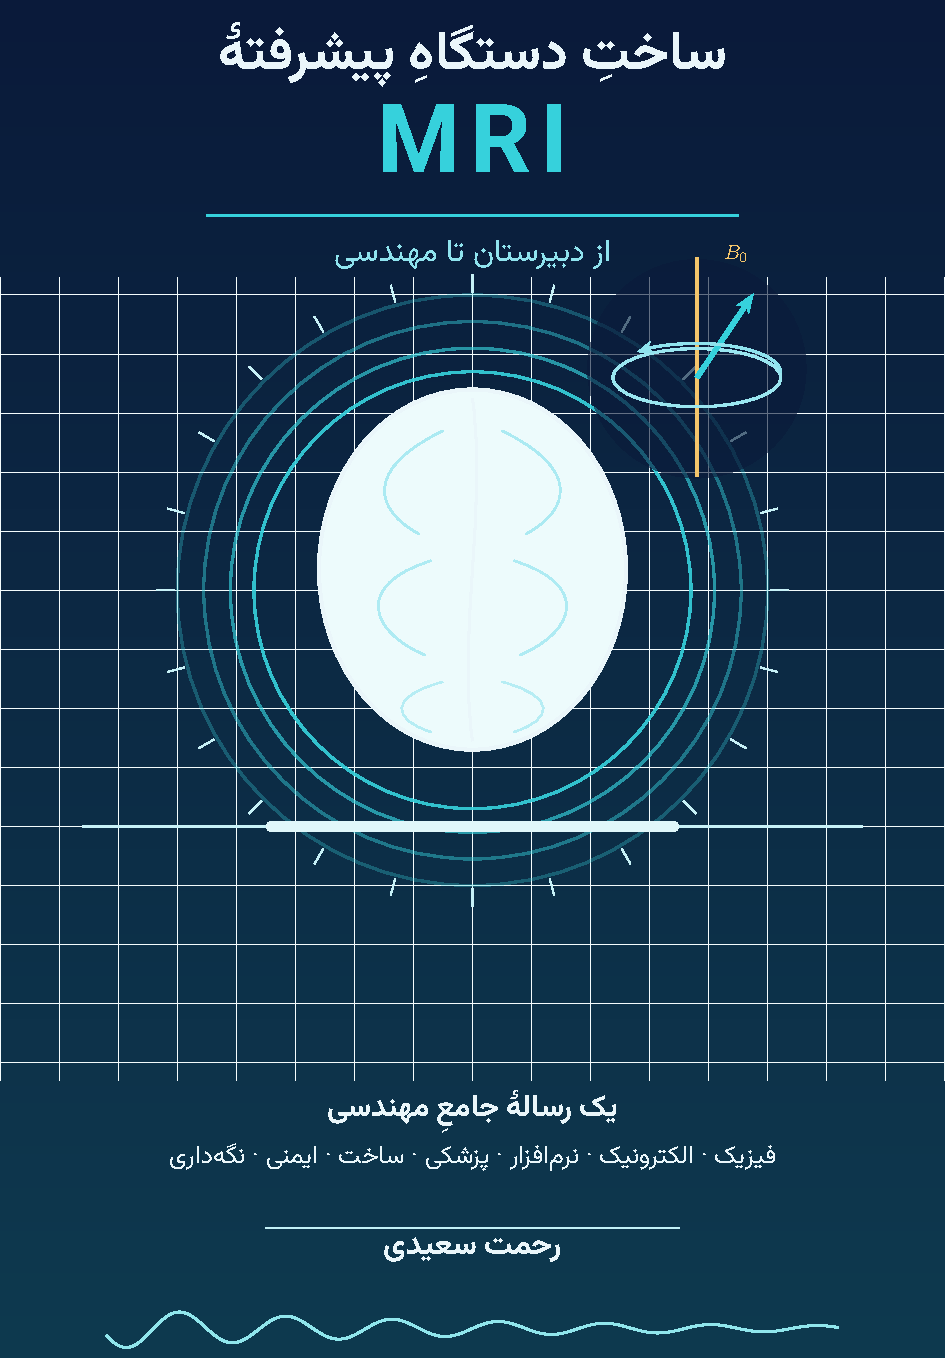
\includepdf[fitpaper=true]{cover/cover.pdf}}

% --- Table of contents: number column width (RTL) ----------------------------
% In the RTL ToC, multi-part section numbers (e.g. "78.10") are wider than the
% default reserved slot and collide with the Persian heading text. Reserve a
% wider, per-level number column via KOMA's tocbasic so the number and title
% never overlap. (Chapter numbers reach 77; section numbers reach NN.NN.)
% ToC display depth (chapter+section only) is controlled by `toc-depth` in
% _quarto.yml, which Quarto emits as \setcounter{tocdepth}{..} after this file.
\DeclareTOCStyleEntry[numwidth=2.8em]{tocline}{chapter}
\DeclareTOCStyleEntry[numwidth=3.6em]{tocline}{section}
\DeclareTOCStyleEntry[numwidth=4.4em]{tocline}{subsection}

% --- Code blocks render LEFT-TO-RIGHT (English code). -----------------------
% Handled in theme/ltr.lua: each code block is wrapped from the OUTSIDE in the
% LTR `english` language (\begin{otherlanguage}{english} ... around the whole
% `Shaded` box), which both fixes reading order and left-aligns the block,
% without disturbing the framed/verbatim internals. Inline `code` is wrapped
% in \babelsublr there as well.

% --- Mathematics stays left-to-right automatically inside math mode. --------
% unicode-math is optional; enable only if a specific math font is required.
% \usepackage{unicode-math}
% \setmathfont{Latin Modern Math}
